\section{Brownian motion}
	While the elementary kinetic theory successfully explains many observed properties of gases, the first experimental evidence for the existence of molecules and their continuous chaotic motion was provided by Robert Brown in 1827. He observed the motion of very small pollen grains suspended in water using a high power microscope. The suspended particles were seen to move completely haphazardly and execute perpetual movement. This irregular motion of the particles is termed \emph{Brownian motion}.
	\begin{figure}[h!]
		\centering
		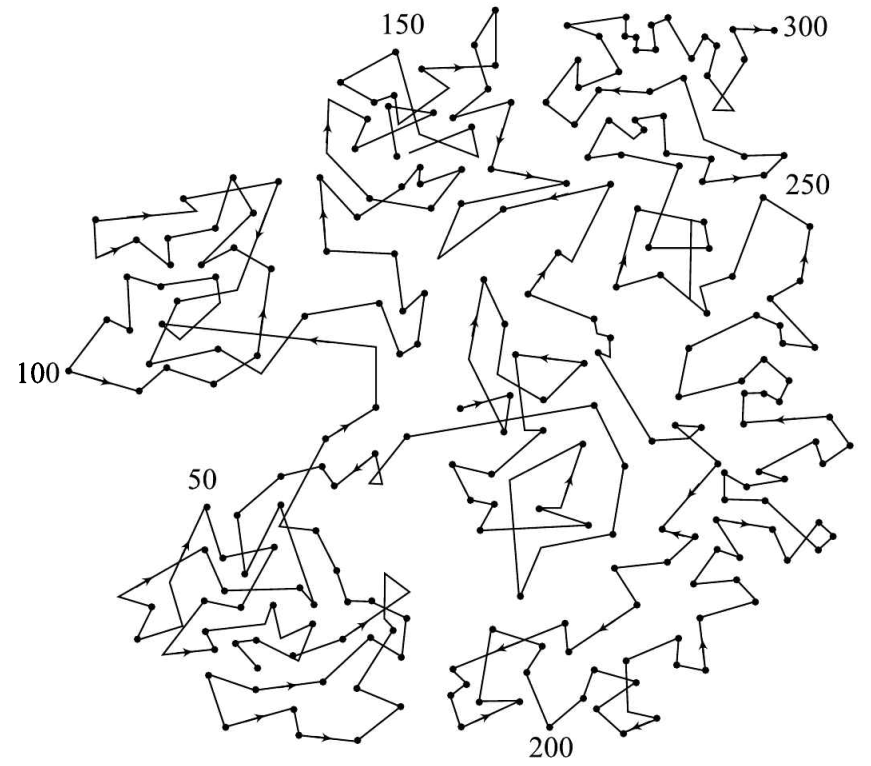
\includegraphics[width=0.7\textwidth]{figures/fig_brownian-motion.png}
	\end{figure}
	
	\subsection{Characteristics of Brownian motion}
		The observed characteristics of Brownian motion are as follows:
		\begin{enumerate}
			\item The motion is continuous, completely random and irregular.
			\item No two particles execute the same motion.
			\item Smaller particles execute faster and hence more noticeable motion.
			\item The motion becomes more vigorous and lively when temperature is increased or a less viscous liquid is taken.
			\item The movement is about the same in all directions.
			\item The motion is independent of external influences.
		\end{enumerate}
		
	\subsection{Qualitative explanation for Brownian motion}
		The discovery of Brownian motion puzzled scientists for a long time, and at first, it was regarded as a property of organic matter. However, experiments proved conclusively that the motion is not due to any biological or chemical factor, establishing that small particles of inorganic matter suspended in both liquids and gases also execute Brownian motion. After discarding explanations based on surface tension, temperature non-homogeneity, and chemical or electrical action, it was proposed that Brownian motion is due to the bombardment of suspended particles by the molecules of the surrounding fluid.
		
		For bigger particles, the forces due to molecular impacts almost completely balance. However, for smaller particles, molecular impacts do not exactly balance and the unbalanced force makes them move in a random manner.
		
		Brownian motion provides a very useful picture of the gaseous state. One can suppose that like Brownian particles, gas molecules are in random motion and frequently collide with each other. Brownian motion is readily observed in gases because intermolecular forces are negligibly small.
		
		\subsubsection{Einstein's theory (1905)}
			\begin{itemize}
				\item Approaches Brownian motion through statistical mechanics and thermodynamics, linking microscopic particle behavior to macroscopic fluid properties.
				\item Models the irregular movement as a random walk and connects it to the laws of diffusion.
				\item Establishes that the mean squared displacement of a particle is directly proportional to both the absolute temperature and the elapsed time ($\expval{x^2}=2Dt$), offering a direct way to calculate Avogadro's number and prove the existence of atoms.
			\end{itemize}
		
		\subsubsection{Langevin's theory (1908)}
			\begin{itemize}
				\item Analyzes the phenomenon through direct Newtonian mechanics, focusing on the dynamic trajectory of a single particle.
				\item Models the interactions using Newton's second law by splitting the total force from the fluid into two distinct components: a macroscopic viscous drag that continuously resists motion, and a rapidly fluctuating, random stochastic force caused by molecular collisions.
				\item Arrives at the same physical conclusions as Einstein regarding particle displacement, but does so through a much more direct, mechanical framework that became the foundation for modern stochastic differential equations.
			\end{itemize}